\Opensolutionfile{ans}[ans/ansCD2D1-3-4]
\begin{dang}{Bài toán tham số về Max - Min}
\end{dang}
\paragraph{Các ví dụ}
\begin{vd}%Câu 1.%[2D1K3-1]
	Tìm giá trị thực của tham số $a$ để hàm số $f(x)=-x^3-3x^2+a$ có giá trị nhỏ nhất trên đoạn $[-1;1]$ bằng $0$.
	\loigiai{
		Đạo hàm $f'(x)=-3x^2-6x\Rightarrow f'(x)=0\Leftrightarrow\hoac{&x=0\in[-1;1]\\&x=-2\notin[-1;1].}$ \\
		Ta có $\heva{&f(-1)=a-2\\&f(0)=a\\&f(1)=a-4}\Rightarrow\min\limits_{[-1;1]} f(x)=f(1)=a-4$.\\
		Theo bài ra: $\min\limits_{[-1;1]} f(x)=0\Leftrightarrow a-4=0\Leftrightarrow a=4$.}
\end{vd}
\begin{vd}%Câu 2.%[2D1K3-1]
	Cho hàm số $f(x)=\dfrac{x-m^2+m}{x+1}$ với $m$ là tham số thực. Tìm tất cả các giá trị của $m$ để hàm số có giá trị nhỏ nhất trên đoạn $[0;1]$ bằng $-2$.
	\loigiai{
		Đạo hàm $f'(x)=\dfrac{m^2-m+1}{(x+1)^2}>0,\forall x\in[0;1]$.\\
		Suy ra hàm số $f(x)$ đồng biến trên $[0;1]\Rightarrow\min\limits_{[0;1]} f(x)=f(0)=-m^2+m$.\\
		Theo bài ra: $\min\limits_{[0;1]} f(x)=-2\Leftrightarrow-m^2+m=-2\Leftrightarrow m^2-m-2=0\Leftrightarrow\hoac{&m=-1\\&m=2.}$	
	}
\end{vd}
\begin{vd}%Câu 3.%[2D1K3-1]
	Tìm tất cả giá trị của $m$ để giá trị nhỏ nhất của hàm số $f(x)=\dfrac{2x+m-1}{x+1}$ trên đoạn $[1;2]$ bằng $1$.
	\loigiai{
		Ta có $f'(x)=\dfrac{3-m}{(x+1)^2}$.\\
		Nếu $m<3$: $f'(x)=\dfrac{3-m}{(x+1)^2}>0$ nên hàm số đồng biến trên $[1;2]\Rightarrow\min\limits_{[1;2]} f(x)=f(1)=1$.\\
		Vậy $\min\limits_{[1;2]} f(x)=1\Leftrightarrow f(1)=1\Leftrightarrow\dfrac{m+1}{2}=1\Leftrightarrow m=1$ (nhận).\\
		Nếu $m>3$: $f'(x)=\dfrac{3-m}{(x+1)^2}<0$ nên hàm số nghịch biến trên $[1;2]\Rightarrow\min\limits_{[1;2]} f(x)=f(2)=1$. \\
		Vậy $\min\limits_{[1;2]} f(x)=1\Leftrightarrow f(2)=1\Leftrightarrow\dfrac{3+m}{3}=1\Leftrightarrow m=0$ (loại).\\
		Kết luận: $m=1$.
	}
\end{vd}
% \begin{vd}%Câu 4.%[2D1K3-1]
% 	Tìm các giá trị của tham số $m$ sao cho giá trị lớn nhất của hàm số $y=\left|x^2-2x+m\right|$ trên đoạn $[-1;2]$ bằng $5$.
% 	\loigiai{
% 		Xét hàm số $f(x)=x^2-2x+m$ trên đoạn $[-1;2]$, ta có $f'(x)=2(x-1)$ và $f'(x)=0\Leftrightarrow x=1$.\\
% 		Vậy $\max\limits_{[-1;2]} y=\max\limits_{[-1;2]}\left|f(x)\right|=\max\left\{\left|f(-1)\right|;\left|f(1)\right|;\left|f(2)\right|\right\}=\max\left\{|3+m|;|m-1|;|m|\right\}$.\\
% 		TH1. Với $\max\limits_{[-1;2]} y=|m-1|$, ta có $\heva{&|m-1|\geq|m+3|\\&|m-1|\geq|m|\\&|m-1|=5}\Leftrightarrow\heva{&|m-1|\geq|m+3|\\&|m-1|\geq|m|\\&m=-4\vee m=6}\Leftrightarrow m=-4$.\\
% 		TH2. Với $\max\limits_{[-1;2]} y=|m+3|$, ta được $\heva{&|m+3|\geq|m-1|\\&|m+3|\geq|m|\\&|m+3|=5}\Leftrightarrow\heva{&|m+3|\geq|m-1|\\&|m+3|\geq|m|\\&m=2\vee m=-8}\Leftrightarrow m=2$.\\
% 		TH3. Với $\max\limits_{[-1;2]} y=|m|$, ta được $\heva{&|m|\geq|m-1|\\&|m|\geq|m+3|\\&|m|=5}\Leftrightarrow\heva{&|m|\geq|m-1|\\&|m|\geq|m+3|\\&m=5\vee m=-5}$ (vô nghiệm).\\
% 	Kết luận: $m\in\{-4,2\}$.
% 	}
% \end{vd}
\paragraph{Câu hỏi trắc nghiệm}
\begin{ex}%Câu 1.%[2D1K3-1]
	Cho hàm số $f(x)=x^3+\left(m^2+1\right)x+m^2-2$ với $m$ là tham số thực. Tìm tất cả các giá trị của $m$ để hàm số có giá trị nhỏ nhất trên đoạn $[0;2]$ bằng $7$. 
	\choice
	{$m=\pm 1$}
	{$m=\pm\sqrt{7}$}
	{$m=\pm\sqrt{2}$}
	{\True $m=\pm 3$}
	\loigiai{
		Đạo hàm $f'(x)=3x^2+m^2+1>0,\forall x\in\mathbb{R}$.\\
		Suy ra hàm số $f(x)$ đồng biến trên $[0;2]\Rightarrow\min\limits_{[0;2]} f(x)=f(0)=m^2-2$.\\
		Theo bài ra: $\min\limits_{[0;2]} f(x)=7\Leftrightarrow m^2-2=7\Leftrightarrow m=\pm 3$.}
\end{ex}
\begin{ex}%Câu 2.%[2D1K3-1]
	Cho hàm số $f(x)=\dfrac{x-m^2}{x+8}$ với $m$ là tham số thực. Tìm giá trị lớn nhất của $m$ để hàm số có giá trị nhỏ nhất trên đoạn $[0;3]$ bằng $-2$. 
	\choice
	{\True $m=4$}
	{$m=5$}
	{$m=-4$}
	{$m=1$}
	\loigiai{
		Đạo hàm $y'=\dfrac{8+m^2}{(x+8)^2}>0,\forall x\in[0;3]$.\\
		Suy ra hàm số $f(x)$ đồng biến trên đoạn $[0;3]\Rightarrow\min\limits_{[0;3]} f(x)=f(0)=-\dfrac{m^2}{8}$.\\
		Theo bài ra: $\min\limits_{[0;3]} f(x)=-2\Leftrightarrow-\dfrac{m^2}{8}=-2\Leftrightarrow m=\pm 4$.\\ Do đó giá trị $m$ lớn nhất là $m=4$.}
\end{ex}
\begin{ex}%Câu 3.%[2D1K3-1]
	Cho hàm số $y=\dfrac{x+m}{x+1}$. Với tham số $m$ bằng bao nhiêu thì thỏa mãn $\min\limits_{[1;2]} y+\max\limits_{[1;2]} y=\dfrac{16}{3}$. 
	\choice
	{$m=0$}
	{$m=2$}
	{$m=4$}
	{\True $m=5$}
	\loigiai{
		Đạo hàm $f'(x)=\dfrac{1-m}{(x+1)^2}$.\\
		Suy ra hàm số $f(x)$ là hàm số đơn điệu trên đoạn $[1;2]$ với mọi $m\neq 1$.\\
		Khi đó $\min\limits_{[1;2]} y+\max\limits_{[1;2]} y=f(1)+f(2)=\dfrac{m+1}{2}+\dfrac{m+2}{3}=\dfrac{16}{3}\Leftrightarrow\dfrac{5m}{6}=\dfrac{25}{6}\Leftrightarrow m=5$.}
\end{ex}
\begin{ex}%Câu 4.%[2D1K3-1]
	Cho hàm số $f(x)=\dfrac{2\sqrt{x}+m}{\sqrt{x+1}}$ với $m$ là tham số thực. Tìm tất cả các giá trị của $m>1$ để hàm số có giá trị lớn nhất trên đoạn $[0;4]$ nhỏ hơn $3$. 
	\choice
	{$m\in(1;3)$}
	{$m\in\left(1;3\sqrt{5}-4\right)$}
	{\True $m\in(1;\sqrt{5})$}
	{$m\in(1;3]$}
	\loigiai{
		Đạo hàm $f'(x)=\dfrac{2-m\sqrt{x}}{2(x+1)\sqrt{x(x+1)}}$, $ f'(x)=0\Leftrightarrow\sqrt{x}=\dfrac{2}{m}\Leftrightarrow x=\dfrac{4}{m^2}\in[0;4],\forall m>1$.\\
		Bảng biến thiên
		\begin{center}
			\begin{tikzpicture}[>=stealth]
			\tkzTabInit[nocadre=false,lgt=1,espcl=2.2,deltacl=0.7]{$x$/1.2 ,$f'$/.7,$f$/2.2}
			{$0$ , $\dfrac{4}{m^2}$ , $4$}
			\tkzTabLine{ , + , $0$ , - , }
			\tkzTabVar{-/$f(0)$ , +/$\sqrt{m^2+4}$ , -/$f(4)$}
			\end{tikzpicture}			
		\end{center}
		Suy ra $\max\limits_{[0;4]} f(x)=f\left(\dfrac{4}{m^2}\right)=\sqrt{m^2+4}$.\\
		Vậy ta cần có $\sqrt{m^2+4}<3\Leftrightarrow m<\sqrt{5}\xrightarrow{{m>1}}m\in(1;\sqrt{5})$.}
\end{ex}
\begin{ex}%Câu 5.%[2D1K3-1]
	Cho hàm số $y=x^3-3x+1$. Tìm tìm tập hợp tất cả giá trị $m>0$, để giá trị nhỏ nhất của hàm số trên $\mathscr{D}=[m+1;m+2]$ luôn bé hơn $3$ là 
	\choice
	{\True $(0;1)$}
	{$\left(\dfrac{1}{2};1\right)$}
	{$(-\infty;1)\setminus\{-2\}$}
	{$(0;2)$}
	\loigiai{
		Ta có: $y'=3x^2-3$, $y'=0\Leftrightarrow x=\pm 1$.
		Bảng biến thiên
		\begin{center}
			
\begin{tikzpicture}[>=stealth]
			\tkzTabInit[nocadre=false,lgt=1,espcl=2,deltacl=0.5]{$x$/.7 ,$y'$/.7,$y$/2}
			{$-\infty$ , $-1$ , $1$ , $+\infty$}
			\tkzTabLine{ , + , $0$ , - , $0$ , + , }
			\tkzTabVar{-/$-\infty$ , +/$3$ , -/$-1$ , +/$+\infty$}
			\end{tikzpicture}			
		\end{center}
		Suy ra hàm số đồng biến trên khoảng $(1;+\infty)$.\\
		Trên $D=[m+1;m+2]$ với $m>0$, ta có \[\min\limits_{[m+1;m+2]} y=y(m+1)=(m+1)^3-3(m+1)+1=m^3+3m^2-1.\]
		$\min\limits_{[m+1;m+2]} y<3\Leftrightarrow m^3+3m^2-4<0\Leftrightarrow (m-1)(m+2)^2<0\Leftrightarrow \heva{&m<1\\ &m\neq -2.}$\\
		Kết hợp điều kiện, suy ra $m\in(0;1)$.}
\end{ex}
\begin{ex}%Câu 6.%[2D1K3-1]
	Tìm tất cả các giá trị của $m$ để hàm số $f(x)=\dfrac{mx+1}{x-m}$ có giá trị lớn nhất trên $[1; 2]$ bằng $-2$. 
	\choice
	{$m=-3$}
	{$m=2$}
	{$m=4$}
	{\True $m=3$}
	\loigiai{
		Tập xác định: $\mathscr{D}=\mathbb{R}\setminus\{m\}\Rightarrow m\notin[1; 2]$.\\
		$f'(x)=\dfrac{-m^2-1}{(x-m)^2}<0,\forall x\neq m\Rightarrow\max\limits_{[1; 2]} f(x)=f(1)=\dfrac{m+1}{1-m}$.\\
		Theo đề bài $\max\limits_{[1; 2]} f(x)=-2\Leftrightarrow\dfrac{m+1}{1-m}=-2\Leftrightarrow m+1=2m-2\Leftrightarrow m=3$.}
\end{ex}
\begin{ex}%Câu 7.%[2D1K3-1]
	Cho hàm số $y=f(x)={x+m}{x-1}$. Với tham số $m$ bằng bao nhiêu thì $\min\limits_{[2;4]} y=3$?
	\choice
	{$m=1$}
	{$m=3$}
	{\True $m=5$}
	{$m=-1$}
	\loigiai{
		Đạo hàm $f'(x)=-\dfrac{m+1}{(x-1)^2}$.\\
		TH1. Với $m >-1$ suy ra $f'(x)=-\dfrac{m+1}{(x-1)^2}<0,\forall x\neq 1$ nên hàm số $f(x)$ nghịch biến trên mỗi khoảng xác định. Khi đó $\min\limits_{[2;4]} y=f(4)=\dfrac{m+4}{3}=3\Leftrightarrow m=5$ (chọn).\\
		TH2. Với $m <-1$ suy ra $f'(x)=-\dfrac{m+1}{(x-1)^2}>0,\forall x\neq 1$ nên hàm số $f(x)$ đồng biến trên mỗi khoảng xác định. Khi đó $\min\limits_{[2;4]} y=f(2)=m+2=3\Leftrightarrow m=1$ (loại).}
\end{ex}
\begin{ex}%Câu 8.%[2D1K3-2]
	Cho hàm số $f(x)=\dfrac{x+m}{\sqrt{x^2+1}}$. Tìm tất cả các giá trị của tham số thực $m$ để hàm số đạt giá trị lớn nhất tại điểm $x=1$. 
	\choice
	{$m=2$}
	{\True $m=1$}
	{Không có giá trị $m$}
	{$m=-3$}
	\loigiai{
		Tập xác định $\mathscr{D}=\mathbb{R}$, $f'(x)=\dfrac{1-mx}{\left(x^2+1\right)\sqrt{x^2+1}}$.\\
		Vì hàm số liên tục và có đạo hàm trên $\mathbb{R}$ nên để hàm số đạt giá trị lớn nhất tại $x=1$, điều kiện cần là $f'(1)=0\Leftrightarrow 1-m=0\Leftrightarrow m=1$.\\
		Với $m=1$, ta có $f(x)=\dfrac{x+1}{\sqrt{x^2+1}}$, suy ra $f'(x)=\dfrac{1-x}{\left(x^2+1\right)\sqrt{x^2+1}}$, $f'(x)=0\Leftrightarrow x=1$.\\
		Bảng biến thiên
		\begin{center}
			
\begin{tikzpicture}[>=stealth]
			\tkzTabInit[nocadre=false,lgt=1,espcl=2,deltacl=0.5]{$x$/.7 ,$y'$/.7,$y$/2}
			{$-\infty$ , $1$ , $+\infty$}
			\tkzTabLine{ , + , $0$ , - , }
			\tkzTabVar{-/$-1$ , +/$\sqrt{2}$ , -/$1$}
			\end{tikzpicture}							
		\end{center}
		Vậy hàm số đạt giá trị lớn nhất tại $x=1$ khi $m=1$.}
\end{ex}
\begin{ex}%Câu 9.%[2D1K3-1]
	Tìm tất cả các giá trị thực khác $0$ của tham số $m$ để hàm số $y=\dfrac{mx}{x^2+1}$ đạt giá trị lớn nhất tại $x=1$ trên đoạn $[-2;2]$?
	\choice
	{$m=-2$}
	{$m<0$}
	{\True $m>0$}
	{$m=2$}
	\loigiai{
		Ta có $y'=\dfrac{m\left(1-x^2\right)}{\left(x^2+1\right)^2}$.\\
		Do $m\neq 0$ nên $y'=0\Leftrightarrow x=\pm 1\in[-2;2]$. \\
		Vì hàm số đã cho liên tục và xác định nên hàm số đạt giá trị lớn nhất tại $x=1$ trên đoạn $[-2;2]$ khi và chỉ khi $\heva{&y(1)\geq y(-2)\\&y(1)\geq y(2)\\&y(1)\geq y(-1)}\Leftrightarrow m\geq 0$.\\
		Vậy $m>0$ (do $m\neq 0$).}
\end{ex}
\begin{ex}%Câu 10.%[2D1G3-1]
	Tìm tất cả các giá trị thực của tham số $m$ để hàm số $y=\dfrac{x^2+mx+1}{x+m}$ liên tục và đạt giá trị nhỏ nhất trên $[0;2]$ tại một điểm $x_0\in(0;2)$. 
	\choice
	{\True $0<m<1$}
	{$m>1$}
	{$m>2$}
	{$-1<m<1$}
	\loigiai{
		Điều kiện: $x\neq-m$. Ta có: $y'=\dfrac{x^2+2mx+m^2-1}{(x+m)^2}=\dfrac{(x+m)^2-1}{(x+m)^2}$.\\
		$y'=0\Leftrightarrow(x+m)^2=1\Leftrightarrow\hoac{&x=1-m >-m\\&x=-1-m <-m.}$ \\
		Do hệ số $x^2$ là số dương và theo yêu cầu đề bài ta có bảng biến thiên như sau 
		\begin{center}
			
\begin{tikzpicture}
			\tikzset{double style/.append style = {double distance=2pt}}
			\tikzset{h style/.style = {pattern=north west lines}}
			\tkzTabInit[nocadre,lgt=1.5,espcl=3.5]
			{$x$ /1, $y'$ /1,$y$ /2}
			{$-\infty$,$-1-m$,$-m$,$1-m$,$+\infty$}
			\tkzTabLine{  ,+,z,-,d ,- ,z,+, }
			\tkzTabVar{-/$-\infty$,+/$y_1$,-D+/$-\infty$/$+\infty$,-/$y_2$,+/$+\infty$ }
			\end{tikzpicture}
		\end{center}
		Hàm số đạt giá trị nhỏ nhất tại $x_0=1-m\in(0;2)$ nên $0 <-m+1<2\Leftrightarrow-1<m<1$.\\
		Kết hợp điều kiện để hàm số liên tục trên $[0;2]$ thì $-m\notin[0;2]\Leftrightarrow\hoac{&-m<0\\&-m>2}\Leftrightarrow\hoac{&m>0\\&m <-2.}$ \\
		Vậy $0<m<1$.}
\end{ex}

\Closesolutionfile{ans}